\documentclass[conference]{IEEEtran}
\IEEEoverridecommandlockouts
% The preceding line is only needed to identify funding in the first footnote. If that is unneeded, please comment it out.
\usepackage{cite}
\usepackage{amsmath,amssymb,amsfonts}
\usepackage{algorithmic}
\usepackage{graphicx}
\usepackage{textcomp}
\usepackage{xcolor}
\def\BibTeX{{\rm B\kern-.05em{\sc i\kern-.025em b}\kern-.08em
    T\kern-.1667em\lower.7ex\hbox{E}\kern-.125emX}}

\usepackage[styles]{idrislang}

\newcommand\todo[1]{\textcolor{red}{#1}}
\usepackage{newfloat}
\DeclareFloatingEnvironment[name={Listing}]{codefig}
\usepackage{xcolor}
%\usepackage{caption}
\usepackage{listings}

\definecolor{codegreen}{rgb}{0,0.6,0}
\definecolor{codegray}{rgb}{0.5,0.5,0.5}
\definecolor{codepurple}{rgb}{0.58,0,0.82}
\definecolor{backcolour}{rgb}{0.95,0.95,0.92}

\lstdefinestyle{mystyle}{
    %backgroundcolor=\color{backcolour},   
    commentstyle=\color{codegreen},
    keywordstyle=\color{magenta},
    numberstyle=\tiny\color{codegray},
    stringstyle=\color{codepurple},
    basicstyle=\ttfamily\footnotesize,
    breakatwhitespace=false,         
    breaklines=true,                 
    captionpos=b,                    
    keepspaces=true,                 
    numbers=left,                    
    numbersep=5pt,                  
    showspaces=false,                
    showstringspaces=false,
    showtabs=false,                  
    frame=lines,
    tabsize=2
}

\lstset{style=mystyle}
\usepackage{svg}

\begin{document}

\title{On Applications of Dependent Types to Parameterised Digital Signal
  Processing Circuits \\
\thanks{Funded under EPSRC grant no. EP/N509760/1} }

\author{\IEEEauthorblockN{Craig Ramsay}
\IEEEauthorblockA{
\textit{University of Strathclyde}\\
Glasgow, Scotland \\
\href{craig.ramsay.100@strath.ac.uk}}
\and
\IEEEauthorblockN{Louise H. Crockett}
\IEEEauthorblockA{
\textit{University of Strathclyde}\\
Glasgow, Scotland \\
louise.crockett@strath.ac.uk}
\and
\IEEEauthorblockN{Robert W. Stewart}
\IEEEauthorblockA{
\textit{University of Strathclyde}\\
Glasgow, Scotland \\
r.stewart@strath.ac.uk}
}

\maketitle

\begin{abstract}
  We'll introduce Idris for EEE folks and show where there's a dependently typed
  hole in most hardware description languages, and what sort of signal
  processing circuits we can construct if we had such a language feature.
\end{abstract}

\begin{IEEEkeywords}
dependent types, functional programming, Idris, digital signal processing, field programmable gate arrays  
\end{IEEEkeywords}

\section{Introduction}

Issues we see in describing DSP things generically. VHDL no good, so people used
things like perl to generate vhdl in an unsafe way for ages. The essence of this
technique has been continued with more feature rich HDLs, including those
embedded in Haskell. These languages still rely on the execution of the
designer's software program to generate hardware --- meaning structure and
wordlengths will be evaluated only when the program is called with a specific
set of arguments. Testing is still a big burden here. It's also hard to guage
how well tested a 3rd party IP is... What if we could describe our circuits in
such a way so the compiler can check the circuit structure and wordlengths, even
when these change in non-trivial ways with changes to the parameters?

Dependent types can do this! What are those? Idris is a good shout.

\section{Modelling synchronous circuits in Idris}

In order to model simple circuit behaviour in Idris, a few choices must be considered. Namely,
\begin{enumerate}
\item \emph{How to best represent numeric types} --- \\A raw collection of bits, or
  native integers? How should binary wordlengths be encoded in the types?
\item \emph{How to best model synchronous logic} --- \\Potentially infinite lists of
  descrete-time samples? How do we ensure causality is preserved? Should
  multiple clock domains be supported?
\end{enumerate}

An intuative solution to choice 1) is to expose only a type representing a
single bit (an equivalent of VHDL's \texttt{std\_logic} type) and let the
designer create their own abstractions on top of this, introducing any number of
different arithmetic semantics and representations (unsigned, signed,
fixed-point, binary-coded decimal, for example). In a slightly more idomatic
approach, we opt for the use of a type class for these bit-representable types
(much like the \texttt{Rep} type class used in Kansas Lava\cite{gill_13}). This
provides a formal interface that defines what a type must implement in order to
be bit-representable. An instance of this type class can be written for any
custom type or, importantly, any existing Idris type. The reuse of existing
types is a benefit over simply constructing new data types as collections of
bits directly.

Choice 2) introduces a substantial level of complexity when considering circuit
synthesis --- but much of this can be side-stepped when performing simulation
alone. One long-standing method of modelling synchonous signals is to use
infinite streams where the $k^{th}$ element represents the discrete-time sample
that is stable during the $k^{th}$ clock cycle. This technique can be seen in
various forms in the languages $\mu$FP\cite{ufp}, Kansas Lavas\cite{gill_09},
and C$\lambda$aSH\cite{baaij_15}.

The host language must, generally, have support for lazy evaluation for
definitions of these infinite stream structures. While Idris uses eagar
evaluation by default (unlike Haskell, the host language of
\cite{gill_09,baaij_15}), lazy evaluation is still supported when operating on
explicitly ``lazy'' types.

A final nuance is that it is possible to describe a variety of non-synthesizable
circuits using streams directly. For example:

\begin{itemize}
\item Dropping an element from the stream describes a time advance, and is
  non-causal
\begin{lstlisting}[language=idris]
adv : Stream a -> Stream a
adv x :: xs = xs
\end{lstlisting}
      
\item Some recursive uses of streams would infer circuits with infinite memory
  elements\cite{baaij_15}
\begin{lstlisting}[language=idris]
elephant : a -> Stream a -> Stream a
elephant i (x :: xs) = i :: x :: elephant i xs
\end{lstlisting}
\end{itemize}

These non-synthesizable descriptions can be precluded by hiding the Stream
implementation and only exposing safe, hardware-friendly functions that operate
on these streams --- such as \texttt{delay}, and an functor interface.

Before considering how Idris' dependent types enhance DSP circuit models, it is
worth reiterating that, at the time of writing, this environment only simulates
synchronous circuit behaviour and \emph{does not} synthesize circuits as VHDL or
verilog descriptions. However, circuit synthesis is a promising avenue for
future work given Idris' support for hosting EDSLs, even with their own syntax
overloading\cite{brady_12}.


\section{First steps:\\Minimal Bit Growth for FIR Adder Chains}
\label{sec:fir}

% Talk about direct form FIR filters with diagram
As an introductory example, the consider a direct form Finite Impulse Response
(FIR) filter shown in Figure \ref{fig:fir_direct}. All word lengths have been
annotated, considering the worst-case for each arithmetic operation in
isolation. 

\begin{figure}
  \centering
  \includesvg{img/firworstcase}
  \caption{A direct form FIR filter with worst-case growth along the adder chain}
  \label{fig:fir_direct}
\end{figure}

% Zoom in on adder chain and talk about worst-case bit growth and how this is
% usually a type-level function (different from dependent types!). For known
% coefficients, we can do better here than worst-case growth.

For this trivial example, the input is an 8-bit word, the coefficients are all
5-bit words, and the adder chain produces a 16-bit output. For worst-case bit
growth, the result of the multiplication of an $n$-bit word and an $m$-bit word
is represented as an $[n+m]$-bit word, and the addition of an $n$-bit and an
$m$-bit word is a $[Max(n,m)+1]$-bit word. This sort of growth can be captured
by VHDL designs using generics and \texttt{for generate} statements. (Note that
there is no type inference, however, so the word length of every intermediate
signal must be explicitly defined.). As an introduction to Idris' syntax we
present this worst-case bit growth for arithmetic functions in Listing
\ref{lst:worst_arith}, where the type \texttt{Unsigned n} represents an unsigned
integer of $n$ bits.

\begin{codefig}[h]
  \caption{Worst-case bit growth for binary arithmetic functions}
\begin{lstlisting}[language=idris]
mul : Unsigned n -> Unsigned m -> Unsigned (n+m)
mul a b = a * b

add : Unsigned n -> Unsigned m
   -> Unsigned (max n m + 1)
add a b = a + b
\end{lstlisting}
\label{lst:worst_arith}
\end{codefig}

Each function has a type (after \texttt{:}), and an implementation (after \texttt{=}).
For clarity, the type of the multiplication function, \texttt{mul}, should be
read as ``a function accepting arguments of type \texttt{Unsigned n} and
\texttt{Unsigned m}, and returns a value of type \texttt{Unsigned (n+m)}''.

In the case of the FIR filter presented in Figure \ref{fig:fir_direct}, a circuit can be described with word lengths better than the worst-case for two reasons:

\begin{enumerate}
\item Each arithmetic operation is considered in isolation but repeated
  additions will accumulate any quantisation effects when the true range of a
  number does not align with power of 2 limits. For example, $y$ in Figure
  \ref{fig:fir_direct} will only inhabit values within the range
  $[\![0,2^{14}-1]\!]$, despite its 16-bit annotation.
\item Often the coefficients, $w_n$, will be constant. In this case the bit
  growth due to multiplication should vary with the numerical value of each
  constant coefficient.
\end{enumerate}

Improvement 2) is particularly relevant here, as its solution clearly demands a
language with dependent types --- a term-level value (a coefficient) must be
used to compute a type (the output word length).

% Let's try! Instead of tracking bits, we track the exact range that a signal
% can inhabit. This can be reduced back to an n-bit number using the Rep type
% class. Look at how we do arithmetic with a constant now... this is an example
% of dependent types! Value is lifted up to the type level and we do
% calculations with it.

Now consider how Idris can be applied to these challenges.

\subsection{An Idris Implementation}

Both improvements are facilitated by types that track the integer range each
signal can inhabit, rather than immediately rounding to the number of bits
required (i.e. $\lceil log_2(range) \rceil$). Our implementation of this is the
\texttt{Bounded} type, where a number of type \texttt{Bounded n} is in the
closed interval $[\![0,n]\!]$ (i.e. any value between 0 and $n$, inclusive).
Such a type can implement the \texttt{Rep} type class in order to maintain a
known binary representation, required for ciruit synthesis.

Listing \ref{lst:better_arith} shows two arithmetic functions on
\texttt{Bounded} that help ensure minimum bit growth for the FIR filter example
--- \texttt{mulConst} to multiply a \texttt{Bounded} with a constant, and
\texttt{add} to add two \texttt{Bounded} arguments.

\begin{codefig}[h]
  \caption{Minimum bit growth for \texttt{Bounded} arithmetic functions}
\begin{lstlisting}[language=idris]
mulConst : Bounded n -> (m: Nat) -> Bounded (n*m)
mulConst (B x n) m = B (x*m) (n*m)

add : Bounded n -> Bounded m -> Bounded (n+m)
add (B x n) (B y m) = B (x+y) (n+m)
\end{lstlisting}
\label{lst:better_arith}
\end{codefig}

Paying particular attention to \texttt{mulConst}'s use of dependent types (the
\emph{type} of the output depends on the \emph{value} of an argument), a full
FIR filter circuit can be constructed using these arithmetic functions. At its
core, an FIR is a dot product of $n$ coefficients ($w$) and the last $n$ samples
of a discrete time signal ($x$).

\begin{equation}
  y_{[k]} = \sum_{k=0}^{n} w_k \cdot x_{[n-k]}
\label{eqn:fir}
\end{equation}

To construct the type for the dot product's output, consider the worst-case
magnitude of each term in Equation \ref{eqn:fir}. As the range of $x_{[n]}$ is
constant for all $n$, it can be taken out as a factor:

\begin{equation}
  |y| = |x|\sum_{k=0}^{n} |w_k|
\label{eqn:fir_mag}
\end{equation}

% Now we can continue and build this into an entire FIR structure. Look at types
% first. See how much of the implementation I can include without being scary...

From this, we can deduce that a valid type for the dot product function is
\texttt{Bounded (m * sum ws)}, given a collection of $n$ coefficients,
\texttt{Vect n Nat} called \texttt{ws}, and a collection of $n$ delayed samples
of $x$, \texttt{Vect n (Bounded m)}. Note that \texttt{sum} is an ordinary
function and it is a consequence of dependent types that we can use it to
construct a type for the dot product output. Listing \ref{lst:dot_prod} shows
the implementation of this combinatorial dot product and the FIR model that
``lifts'' this dot product into a \texttt{Stream}, which models synchronous
logic.

\begin{codefig}[h]
  \caption{Dependently typed FIR implementation}
\begin{lstlisting}[language=idris]
dotProd : (ws : Vect n Nat)
       -> Vect n (Bounded m)
       -> Bounded (m * sum ws)
dotProd {n=Z}        _         _        = zeros
dotProd {n=S l} {m} (w :: ws) (x :: xs) =
  let y = add (mulConst x w) (dotProd ws xs)
  in  rewrite dotProdDistrib m w l ws in y

fir : (ws : Vect n Nat)
   -> Stream (Bounded m)
   -> Stream (Bounded (m * sum ws))
fir {n} ws x = liftA (dotProd ws) (window n zeros x)
\end{lstlisting}
\label{lst:dot_prod}
\end{codefig}

Notice that line 7 includes a ``rewrite'' rule that seems extraneous to the
model of the circuit. This acts as a small proof for the Idris compiler,
demonstrating that the implementation does agree with the type we described. The
type of the dot product is defined as in Equation \ref{eqn:fir_mag}, but the
recusive implementation actually describes something with the following type:

\begin{equation}
|y| = |x\cdot w_i|+|x|\sum_{k=i+1}^{n} |w_k|
\end{equation}

The rewrite rule is simply reminding the compiler of the distributive property
of multiplication in order to have the function type check properly.

To summarise this effort, dependent types have been used to implement an FIR
filter in Idris that models \emph{minimal} bit growth (hence minimal resources)
based on the constant values of the provided coefficients. Because the word
lengths/ranges are tracked in the types used in this implementation, the
compiler ensures that our circuit implements the minimal growth at each
arithmetic stage as defined by our specification in Equation \ref{eqn:fir_mag}.
If an implementation does not meet this specification for any single combination
of parameters, this will be caught and manifest as a compliler error.

% OK, why is this better then?

\subsection{Comparisons to existing HDLs}

% VS VHDL & verilog, there is now an implementation that has minimal bit growth.
% Depending on EDA tools, maybe this does get optimised away to match out
% implementation, but think about the design process. We would use this filter
% as one part of a larger DSP chain. After this filter, it's likely we'd want
% resize to keep the wordlengths managable. We either truncate, 100% losing
% precision, or we'd write the weights down and do the exact calculation we've
% just told the Idris compiler to do to find out how many MSBs will be
% uninhabited. Doh. This is quite a clear advantage. We can also use this
% implementation to reason about circuit resource cost and how this varies with
% parameter changes without going through Vivado!

It is worth taking a moment here to compare this dependently typed, minimum bit
growth FIR filter to the implementations possible in other HDLs. It is clear
from this example that modern functional languages are much more expressive than
traditional HDLs, such as Verilog and VHDL. A typical VHDL FIR filter can be
parameterised in terms of the number of coefficients, the word length of the
coefficients, and the input word length. However, the bit growth is likely to be
worse than even the scenario presented in Figure \ref{fig:fir_direct}. Because
of the lack of type inference or type-level generate statements in VHDL, a
common approach is to simply resize all arithmetic stages to match the full
precision output --- heavily relying on synthesis tools to remove unused nets.

Relying on synthesis tools to prune unused nets is often a valid choice,
especially with simple example circuits. However, consider this filter example
in the context of a real design. It is likely that the filter will be just one
part of a larger chain of DSP circuits. At several points along the data path,
the full precision signals will be shortened to avoid excessive resource
usage. In this case, the designer employ multiple strategies:

\begin{itemize}
\item Truncation/rounding of the LSBs --- introducing some quantisation error
\item Removing any uninhabited MSBs --- retaining full precision, but the
  designer needs to manually evaluate Equation \ref{eqn:fir_mag} to identify any
  uninhabited MSBs for their particular set of coefficients.
\end{itemize}

The second option is appealing as it can reduce word lengths without loss in
precision, but it requries extra effort (for each coeffient set!) just to
emulate a guarantee that is provided statically in our Idris implementation.
Beyond this, breaking the reliance on synthesis tools allows the designer to
reason about resource usages from the source descriptions alone --- including
how resource usage mathematically relates to the choice of any input parameters.

% VS other Haskell HDLs: we would need to make word lengths a term-level thing,
% and we'd get no checking from the compiler. Closest is Lava. Can nearly get
% there. Haskell doesn't really have dependent types but we can use singletons.
% We'd be able to implement the same sort of arithmetic stage as seen in Fig
% XX, but when we come to writing the full FIR filter, we need collections of
% singletons and then this gets super messy. Clash has a similar problem with
% collections of singletons because we don't have general recursion -- just a
% fold. So, we need to hold collections of type-level weights. Eugh. Could do
% some risky type level stuff, but that's blergh.
% If we do keep this bit growth at a type level in Idris, then we 
%\begin{enumerate}
%\item compiler verification that we have implemented what we set out to implement (we've got the right word-lengths at each stage), or...
%\item conversely, we can let our implementation be type-directed. At each stage,
%  we infer new wordlengths (or similar) purely by what the types say should
%  happen.
%\item nice environment to reason about circuit resource costs and how they are
%  linked to the parameters... without running through Vivado.
%\end{enumerate}

There are also clear benefits above other modern functional HDLs. The closest
comparison is with the family of HDLs embedded in Haskell, called
Lava\cite{gill_09}. In Lava, a similar circuit can be described using dynamicly
sized lists of bits to represent each word. It is then the execution of a
(software) Haskell program that generates the circuit, since statically sized
structures are required for most hardware descriptions. In this case, the output
circuit \emph{might} be equivalent to the Idris implementation, but there are no
guarantees about word lengths checked by the compiler --- this is what we have
addressed with dependent types. Without these compiler checks, there is a large
burden on the developer to provide good evidence of testing. There have been
efforts to introduce a subset of basic dependent types to Haskell, using
singletons, but this is not enough to replicate our Idris
implementation\cite{lindley_13}. The coefficient set is a collection of
potentially different singletons, which then requires heterogeneous collections;
another painful Haskell experience.

\section{Going further:\\Lossless Pruning in CIC Interpolators/Decimators}

Moving away from simple FIR examples now, it is exciting to see a range of other
standard DSP components that place similar (generally unmet) demands on existing
HDLs. One other noteworthy wordlength example cannot even rely on synthesis
tools to mask the rough approximations made with traditional HDLs --- Cascaded
Integrator-Comb (CIC) decimators/integrators.

CIC filters are often employed as a very low resource solution for digital
decimation or interpolation. CIC decimators consist of a chain of $N$ integrator
stages, followed by a $\frac{1}{R}$-rate down-sampler, followed by $N$ comb
stages with a differential delay of $M$. Figure \ref{fig:cic} shows an example
CIC decimator with $R=8$, $N=3$ and $M=1$.

\begin{figure}
  \centering
  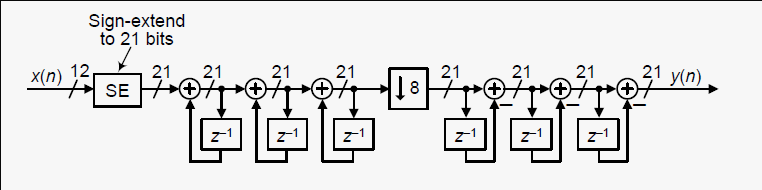
\includegraphics[width=\linewidth]{img/cic_draft}
  \caption{A CIC decimator without pruning. ($R=8$, $N=3$ and $M=1$)}
  \label{fig:cic}
\end{figure}

In Hogenauer's original paper on CIC filters\cite{hogenauer_81}, a register
pruning technique is discussed. Equations are derived that describe the mean
error and variance introduced by truncation at each stage. It is suggested that
given a desired output word length, a legitimate design choice is to prune the
word lengths of all previous stages as much as possible without accumulating an
error greater than that introduced by the final rouding/truncation. This choice
results in the following equation for the number of LSBs to discard at the
$j^{th}$ stage.

\begin{equation}
  B_j = {\Bigg \lfloor} -\log_2F_j + \log_2\sigma_{T_{2N+1}} +\frac{1}{2}\log_2\frac{6}{N} {\Bigg \rfloor}
  \label{eqn:cic_bj}
\end{equation}

where $F_j$ is the variance error gain for the $j^{th}$ stage,
$\sigma_{T_{2N+1}}$ is the total variance at the output due to truncation, and
$N$ is the number of stages. Note that the first two terms have complex
definitions of their own, including cases, sums, exponentials, and binomial
coefficients\cite{hogenauer_81}.

Because the pruned bits at each stage are contain information (we are discarding
these within our own design constraints for error variance), synthesis tools
cannot perform an equivalent optimisation given an un-pruned description. This
section continues by demonstrating how dependent types are used to concisely
describe a fully parameterised, pruned CIC decimator. The conciseness is, in
part, thanks to Idris having a single language that can be used at the
term-level and the type-level -- so all language constructs can be used to
implement Equation \ref{eqn:cic_bj}, and then this function can be used to
direct the type of each stage in a CIC implementation.

\subsection{An Idris Implementation}

Listing \ref{lst:cic_bj} shows the top-level implementation of Equation
\ref{eqn:cic_bj}, after the application of several logarithmic identities to
avoid rounding errors with an integer implementation of $\log_2$.

\begin{codefig}[h]
  \caption{Implementation of Equation \ref{eqn:cic_bj} bit pruning calculation}
\begin{lstlisting}[language=idris]
bj : (r : Nat)   -> (n : Nat)    -> (m : Nat)
  -> (bin : Nat) -> (bout : Nat) -> (j : Nat)
  -> Nat
bj r n m bin bout j =
  flog2Approx $ sigmaT2n1 r n m bin bout
              * (sqrt $ 6.0 / (cast n))
              / (fj r n m j)
\end{lstlisting}
\label{lst:cic_bj}
\end{codefig}

As well as the stage parameter $j$, all CIC parameters are present: the rate
change ($R$), the number of stages ($N$), the differential comb delay ($M$), and
input/output word lengths. Another function \texttt{prunej} inverts
\texttt{bj} to give the number of bits to retain, rather than discard. This
function can now be lifted up to the type definition of a CIC decimator circuit
to help the compiler confirm that each CIC stage is pruned to meet the error
variance design constraint.

\begin{codefig}[h]
  \caption{Type definitions for CIC decimator}
\begin{lstlisting}[language=idris]
-- Internal recursive step
cicDecimateRec :
     (r : Nat)   -> (n : Nat)    -> (m : Nat)
  -> (bin : Nat) -> (bout : Nat) -> (j : Nat)
  -> Stream (Unsigned (prunej r n m bin bout 0))
  -> Stream (Unsigned (prunej r n m bin bout (S j)))
cicDecimateRec r n m bin bout j xs = ?omitted1

-- Top-level CIC
cicDecimate : (r : Nat) -> (n : Nat) -> (m : Nat)
           -> Stream (Unsigned bin)
           -> Stream (Unsigned bout)
cicDecimate {bin} {bout} r n m xs = ?omitted2
\end{lstlisting}
\label{lst:cic_types}
\end{codefig}

Only the type definitions are shown above, but the full CIC decimator
implementation is available at \cite{ramsay_20_gh}.

While this is another example focusing on computing type-level word lengths,
these techniques can be directly applied to many other type-level constructs ---
including circuit topology. It is then only a small leap to apply these
techniques to write type-safe descriptions other DSP circuits. For example,
capturing the structural complexity in Multiple Constant Multiplier blocks, such
as those described by the RAG-n algorithm\cite{dempster_95}.

\subsection{Comparisons to existing HDLs}

This gives us the same advantages over VHDL as the FIR example in section
\ref{sec:fir}, but with the additional distinction that the limitations of
traditional HDLs cannot be partly mitigated by optimisations built into
synthesis tools.

In comparison to HDLs embedded in Haskell, such as Lava, a similar structure may
be technically realisable with type-level functions and singletons. However,
Haskell does not offer the luxury of one rich language that applies to both the
term and type levels. Because of this, the type-level function required to
represent Equation \ref{eqn:cic_bj} (including conditionals, sums, exponentials
and binomial coefficients) would prove to be a painful excursion.

\section{Conclusions}

TODO!

There are common DSP circuits that clearly benefit from them

\section*{Acknowledgment}

The authors would like to thank Xilinx for supplying hardware and EDA tools for
this project. We acknowledge funding for Craig Ramsay under EPSRC grant no.
EP/N509760/1.

\bibliographystyle{IEEEtran}
\bibliography{references} 

\end{document}
